\documentclass[12pt]{article} 

\title{Modelagem em multithread da interação entre colônias de formiga} 
\author{Germano Andrade, João Alcindo e Tiago da Silva} 
\date{\today} 

% language 
\usepackage[portuguese]{babel} 
% general packages 
\usepackage{amssymb} 
\usepackage{amsmath} 
\usepackage{amsthm} 
\usepackage{amsfonts} 
\usepackage{enumitem} 
\usepackage{tabularx} 

% figures 
\usepackage{graphicx} 
\usepackage{tikz} 
\usepackage{tkz-graph} 
\usetikzlibrary{arrows} 
% \usetikzlibrary{calc} 

% theorems environment 
\let \eps \epsilon 
\usepackage{fullpage} 

\newtheorem{theorem}{Teorema} 
\newtheorem{proposition}{Proposição} 

\theoremstyle{definition} 
% \newtheorem{problem}{Exercício} 
\newtheorem{definition}{Definição} 
\newtheorem{lemma}{Lema} 
\newtheorem*{description*}{Problema} 

\SetVertexNormal[Shape      = circle, 
                 LineWidth  = 2pt]
\SetUpEdge[lw         = 1.5pt]

\newcommand\exercisea{\@alpha{a, b, d}}  

\newtheorem{innercustomgeneric}{\customgenericname}
\providecommand{\customgenericname}{}
\newcommand{\newcustomtheorem}[2]{%
  \newenvironment{#1}[1]
  {%
   \renewcommand\customgenericname{#2}%
   \renewcommand\theinnercustomgeneric{##1}%
   \innercustomgeneric
  }
  {\endinnercustomgeneric}
}
\newcustomtheorem{problem}{Exercício}
 
\begin{document}  
	 
\maketitle  
\tableofcontents 

\section{Introdução} 

Neste documento, vamos descrever os aspectos que enformaram nossas implementações e caracterizaram as nossas decisões de modelagem; contemplaremos, além disso, situações tremendamente atribuladas que caracterizaram tanto a implementação serial -- em uma thread -- quanto a multithread deste sistema. Na seção seguinte, portanto, introduzimos os atributos gerais de nosso programa, enfatizando como os agentes -- as formigas, os formigueiros, as comidas e os objetos subjacentes, como os mapas e as coordenadas -- foram desenhados, e apontando, também, para a contemplação dos mecanismos que ensejam sua interação. 

Na seção subsequente, vislumbramos os alicereces que culminaram na versão mulithread do programa, explicitando a utilização de variáveis de exclusão mútua, de variáveis de condição e de semáforos com o objetivo de lograr as idiossincrasias inconvenientes das programação paralela, como as condições de corrida e a inanição (\textit{starvation}). 

\section{Desenho dos agentes} 

A simulação da interaçao entre formigueiros contempla, neste cenário, múltiplos agentes; em um momento inicial, portanto, é importante que os caracterizemos, garantindo que eles possam interagir consistentemente durante a simulação. Em nossa implementação, em particular, identificamos cada agente com uma classe; alguns gozam de múltiplas instâncias (como o agente \texttt{Ant}, formiga), e outros, não (como o agente \texttt{Map}, mapa). Explicitamente, introduzimos as classes 

\begin{enumerate} 
	\item \texttt{Anthill}, formigueiro, 
	\item \texttt{Ant}, formiga, 
	\item \texttt{Food}, comida, 
	\item \texttt{Map}, mapa e 
	\item \texttt{Tile}, azulejo (ou, equivalentemente, coordenada); 
\end{enumerate} 

\noindent elas estão, assim, descritas na Figura~\ref{fig:siml}. Perceba, logo, que as formigas estão amarradas ao formigueiro e, além disso, interagem com ele, incrementando o seu armazém de alimento; em contraste, a interação entre as formigas e a comida consiste no decremento de um atributo -- o volume da instância de comida; por outro lado, as formigas não modificam, objetivamente, os atributos das coordenadas do mapa -- eles que, na verdade, rastreiam, em uma tabela hash (em que as chaves correspondem aos nomes dos formigueiros) de pilhas, as formigas depositadas neles em cada iteração. Esta é, aliás, a interação mais crucial da simulação: as formigas se movem pelo mapa, identificam a comida, a capturam e, em um deslocamento para o formigueiro, incrementam o seu armazenamento de alimento. Nestas condições, o movimento das formigas é delicado; ele é, desta maneira, o tópico da seção seguinte. 

\begin{figure} 
	\centering 
	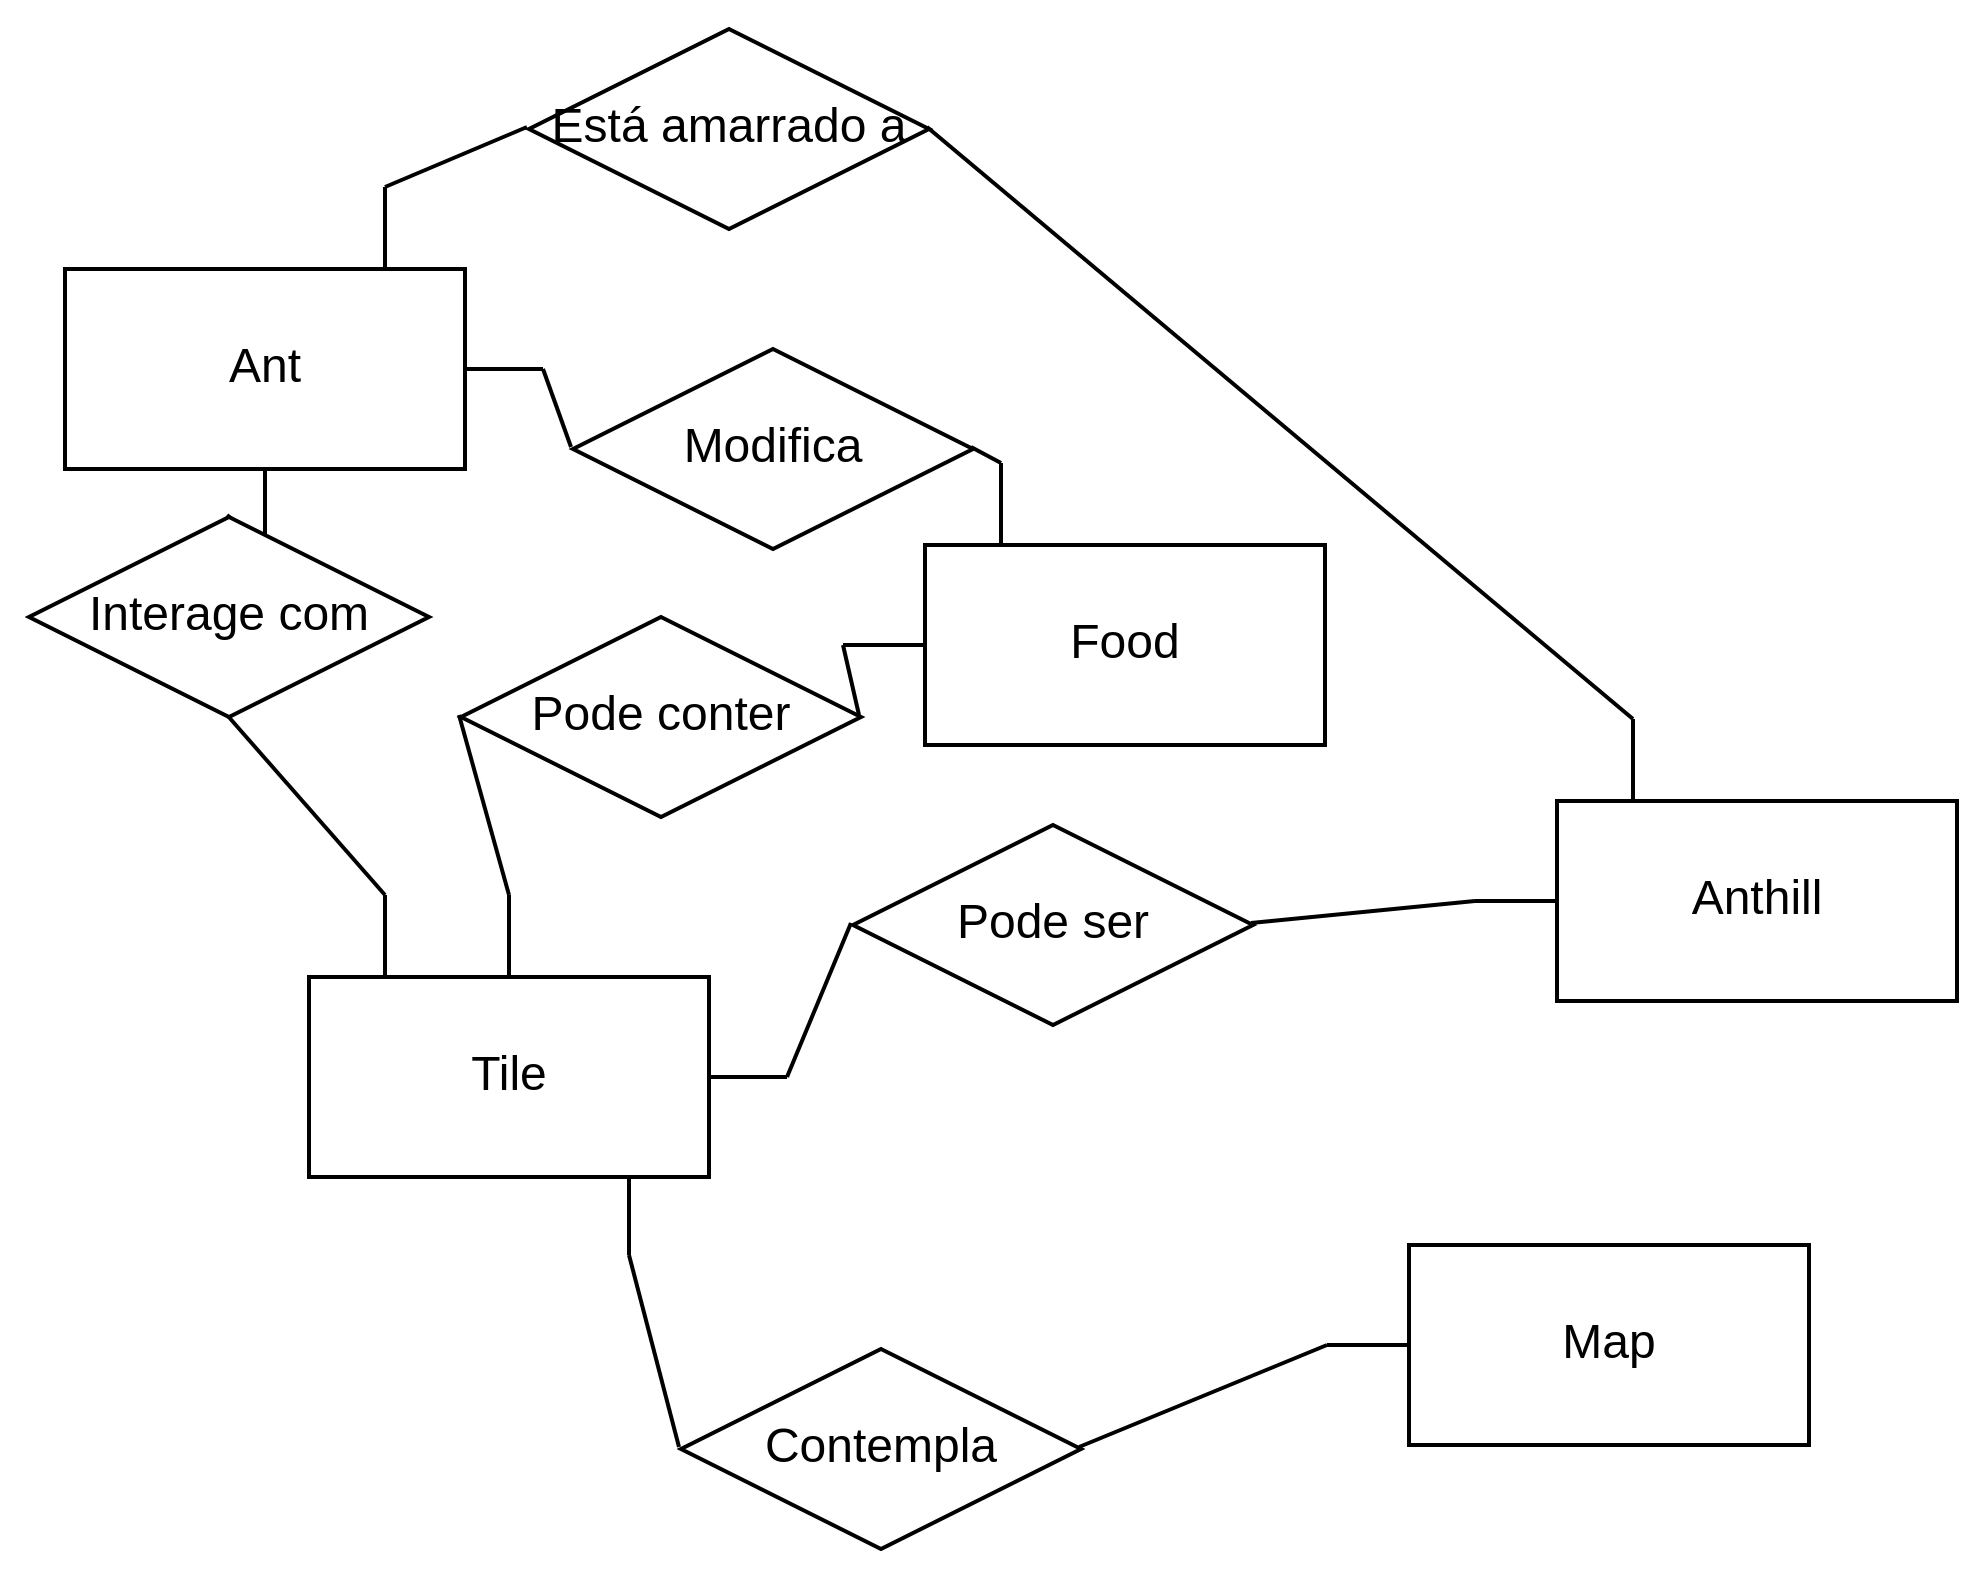
\includegraphics[width = \textwidth]{image.png} 
	\caption{Modelagem e interação dos agentes na simulação.} 
	\label{fig:siml} 
\end{figure} 

\subsection{Movimento das formigas} 

Em cada iteração, há incisivamente um tripleto de ações que as formigas podem executar: ou elas se movem aleatoriamente (método \texttt{moveRandomly}), ou elas se direcionam ao formigueiro (método \texttt{moveToColony}), ou elas procuram o alimento (método \texttt{moveToFood}; elas podem, também, entrar em combate; descreveremos, mais tarde, nossa aproximação para isso). Vislumbramos, nos itens seguintes, cada um desses movimentos. 

\begin{enumerate} 
	\item \texttt{moveRandomly}. No movimento aleatório, identificamos as coordenadas em que a formiga está e, em seguida, capturamos seus vizinhos\footnote{Que não contêm alimento; as formigas não interagem com estes azulejos -- elas modificam as instâncias da classe \texttt{Food} depositadas neles.}, verificando, importantemente, a sua existência (com esse objetivo, o método \texttt{getTile}, da classe \texttt{Map}, levanta uma exceção \texttt{BorderError}, sinalizando que o programa está acessando uma coordenada que transcende as bordas do mapa; o tratamento desta exceção, assim, garante a consistência da identificação das coordenadas vizinhas). Escolhemos, então, uma coordenada aleatoriamente; a probabilidade de uma instância ser escolhida é diretamente proporcional à quantidade de feromônio que ela contém\footnote{Encetamos, para isso, gerando uma variável aleatória uniformemente distribuída no intervalo unitário da reta real; instanciamos, também, uma \texttt{array} com as somas acumuladas das quantidades de feromônios (mais um; por exemplo, um objeto com um feromônio teria peso igual a dois, e um com dois, igual a três) em cada coordenada, \texttt{cumSum}. Aplicamos, então, uma divisão de cada elemento de \texttt{cumSum} pela quantidade total de fermônios nas vizinhanças, e verificamos, assim, o intervalo correspondente à variável aleatória uniforme, que equivale à nossa escolha aleatória.} (a liberação de feromônios é contemplada na seção seguinte). 
	\item \texttt{moveToColony}. Equipadas com alimento, as formigas se direcionam ao formigueiro -- elas têm a informação de sua localização. Elas executam, para isso, um movimento retilíneo, implementado como uma adaptação do algoritmo de Breseham: inicialmente, traçamos, no plano cartersiano, o segmento que amarra a coordenada atual da formiga à de seu formigueiro; na etapa subsequente, computamos a coordenada vizinha da formiga mais próxima deste segmento, e a movemos nesta direção.  
	\item \texttt{moveToFood}. As formigas envisionam, em seu movimento, coordenadas a uma distância caracterizada pelo atributo -- do mapa; todas as formigas, em todos os formigueiros, gozam de campos de visão idênticos (contudo, poderíamos modificar a função que identifica instâncias de \texttt{Food} nas vizinhanças e distinguir a busca por comida para cada formiga -- escolhemos, neste sentido, o desenho mais parcimonioso) --; portanto, elas podem verificar se há alimentos e executar um movimento informado. Neste caso, com as restrições de acesso simultâneo aos alimentos, este ``movimento informado" pode, com efeito, consistir em aguardar e, possivelmente, lutar.  
\end{enumerate} 

Em cada iteração da simulação, assim, cada formiga executa um movimento condicional ao seu estado atual: se ela estiver equipada com comida, ela, incondicionalmente ao seu ambiente, ao formigueiro; se não, ela escaneia o ambiente que a entorna e verifica se há alimentos -- se houver, ela se direciona a eles e, se não, ela se movimenta aleatoriamente. Em algumas circunstâncias, ela escolhe lutar; postergamos a descrição desta ação, contudo, para as seções seguintes. Na seção seguinte, caracterizamos o movimento de formigas com comida e a introdução de feromônios. 

\subsection{Liberação de feromônios} 

Quando capturam alimentos, as formigas se direcionam impetuosamente ao seu formigueiro; em cada movimento, contudo, elas liberam feromônios (\texttt{releasePheromone}; este é um dos métodos da classe \texttt{Ant}) com o objetivo de sinalizar a outras formigas (possivelmente, de outros formigueiros) que existe um caminho, nas proximidades, para uma instância de alimento. Estes feromônios, \texttt{struct Pheromone} com o atributo \texttt{lifetime}, devem ser extraídos do mapa a cada intervalo de iterações; assim, cada instância de \texttt{Tile} contém uma lista, \texttt{pheromones}, de feromônios liberados pelas formigas, que é, em cada iteração, percorrida, ensejando a captura de feromônios mortos -- a intensidade de feromônios nesta coordenada, a propósito, é igual ao tamanho desta lista, que, logo, também é modificada em cada iteração. 

\subsection{Combate entre formigas} 

Em cada iteração, as formigas que não estão direcionando alimentos ao formigueiro podem escolher combater as adversárias; há, neste sentido, um par de cenários em que a luta é executada. Em um deles, a formiga vislumbra, a uma distância (na métrica $L_{1}$) igual a uma unidade, um alimento com volume positivo e, neste caso, seu objetivo é o defender -- neste caso, ela luta deterministicamente, se houver adversários em sua coordenada. Em outro, ela não contempla alimentos em suas vizinhanças e, portanto, ela joga uma moeda justa (utilizamos, neste caso, o algoritmo de amostragem utilizado no movimento aleatório com pesos de feromônios) e executa uma escolha entre um movimento aleatório e uma luta -- se, outra vez, houver adversários. Mais precisamente, ela escolhe guerrear, não lutar, conforme descrevemos nas sentenças seguintes. 

Quando, desta maneira, uma formiga decide lutar, ela executa um ataque coordenado a todas as formigas adversárias em sua coordenada; a probabilidade de que ela vença é, neste caso, proporcional à quantidade de aliadas em sua coordenada. Apesar do ponto culminante desta luta, uma das formigas é \textit{gravemente ferida} e rotulada com o atributo \texttt{isDead}; na iteração seguinte, quando percorrermos a lista de feromônios, também capturaremos as formigas mortas e as extraríremos da simulação. Enfatizamos, aliás, que, mesmo que a rotulação das formigas seja executada em threads distintas, a sua extração é executada na thread principal; isso porque, como elas estão contempladas em um atributo da classe \texttt{Map}, \texttt{allAnts}, precisaríamos garantir que cada thread modificasse este atributo consitentemente, o que, no entanto, é essencialmente equivalente à execução por uma thread (é bastante difícil particionar o tratamento de uma lista entre threads). 

\subsection{Sumário dos agentes} 

A movimentação das formigas, a liberação de feromônios e os aspectos bélicos foram, logo, particularmente inconvenientes, na medida em que eles culminavam na caracterização de ações bastante entrelaçadas -- as formigas modificam as comidas e, também, modificam a si mesmas; a dinamicidade introduzida pelo surgimento da morte foi, também, aflitivo, porque precisávamos, neste caso, ser mais cautelosos na escolha da formiga seguinte a executar o movimento e interagir com o mapa. A propósito, a introdução de aspectos estocásticos na simulação injetou oscilações no sistema que, em alguns cenários, foram inadequadas. 

Tivemos, aliás, confrontos tétricos com a própria linguagem de programação, \texttt{C++}; procedimentos elementares, como o cômputo da distância entre uma coordenada e um segmento, exigiram tremenda introspecção. A implementação de algoritmos multithread, contudo, conformou o epítome de nossas atribulações; nós a descreveremos nas seções seguintes. 

\section{Impressão do mapa no console} 

Neste ínterim, contudo, descrevemos os procedimentos para imprimir o mapa, e suas características, no console; veja, para isso, a Figura~\ref{fig:map}. Antecipamos, aliás, que introduzimos uma variável condicional que controla as threads responsáveis pelos movimentos das formigas quando todas elas tiverem atuado; em seguida, instanciamos outro conjunto de threads para atualizar os atributos do mapa (por exemplo, extrair os feromônios, repor os alimentos ou identificar formigas mortas em combate) -- estes procedimentos estão consolidados no método \texttt{prepareNextIter}, da classe \texttt{Map}. Assim, no estágio seguinte à atualização do mapa, nós o imprimimos, como na Figura~\ref{fig:map}: inicialmente, informamos, para cada colônia, a quantidade de alimentos depositada e a quantidade de formigas vivas; inserimos, então, as coordenadas de cada mapa, com as informações da intensidade de feromônios e da quantidade de formigas. Em maior detalhe, distinguimos a impressão de cada coordenada em um tripleto de categorias, 

\begin{enumerate} 
	\item \textit{andarilhos}, \texttt{|a, p|}, que contempla a quantidade de formigas, \texttt{a}, e de feromônios, \texttt{p}, em cada iteração, 
	\item \textit{formigueuros}, \texttt{|AnthillName, FoodStorage, Ants|}, em que apontamos, sequencialmente, para o nome do formigueiro, a quantidade de alimento armazenado e a quantidade de formigas e 
	\item \textit{comidas}, \texttt{|Food, Volume|}, no qual inserimos, adjacente ao nome \texttt{Food}, a quantidade, em unidades de volume, de alimento disponível. 
\end{enumerate} 

\noindent Estes foram, portanto, os mecanismos que ensejaram a atualização e a impressão do mapa no console; verificaremos, mais tarde, alguns detalhes da implementação multithread. 

\begin{figure} 
	\centering 
	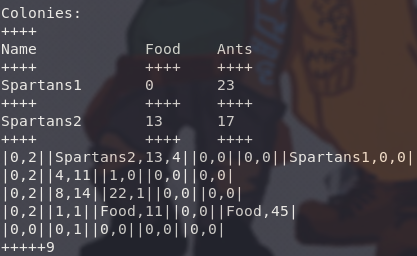
\includegraphics[width = \textwidth]{map.png} 
	\caption{Mapa em que a simulação ocorre.} 
	\label{fig:map} 
\end{figure} 

\section{Implementação multithread} 

Importantemente, encetamos com uma implementação em uma thread; o objetivo disso é garantir que, em circunstâncias com múltiplas threads, os erros sejam culminantes da paralelização, e não idiossincráticos do desenho da simulação. Vamos, desta maneira, descrever, laconicamente, a introdução de múltiplas threads no programa. Escrutinaremos, contudo, a captura de alimento, que, neste caso, consolida inconveniências amarradas fortemente à programação em paralelo. 

Neste sentido, a etapa inicial do programa consiste na inicialização do mapa; precisamos instanciar as coordenadas, os formigueiros e as formigas. Apesar de podermos introduzir múltiplas threads para particionar estas tarefas, escolhemos a decisão mais parcimoniosa e executamos estes procedimentos na thread principal, porque, como esta etapa é executada uma vez, no início da simulação, rotulamos sua paralelização como inapropriada. Em sequência, precisamos executar os procedimentos da simulação -- movimento das formigas e atualização do ambiente -- por uma quantidade de iterações parametrizável; contemplamos, no parágrafo seguinte, esta descrição. 




\end{document} 
